\subsection{The package of Logic}

\begin{figure}[h]
	\centering
	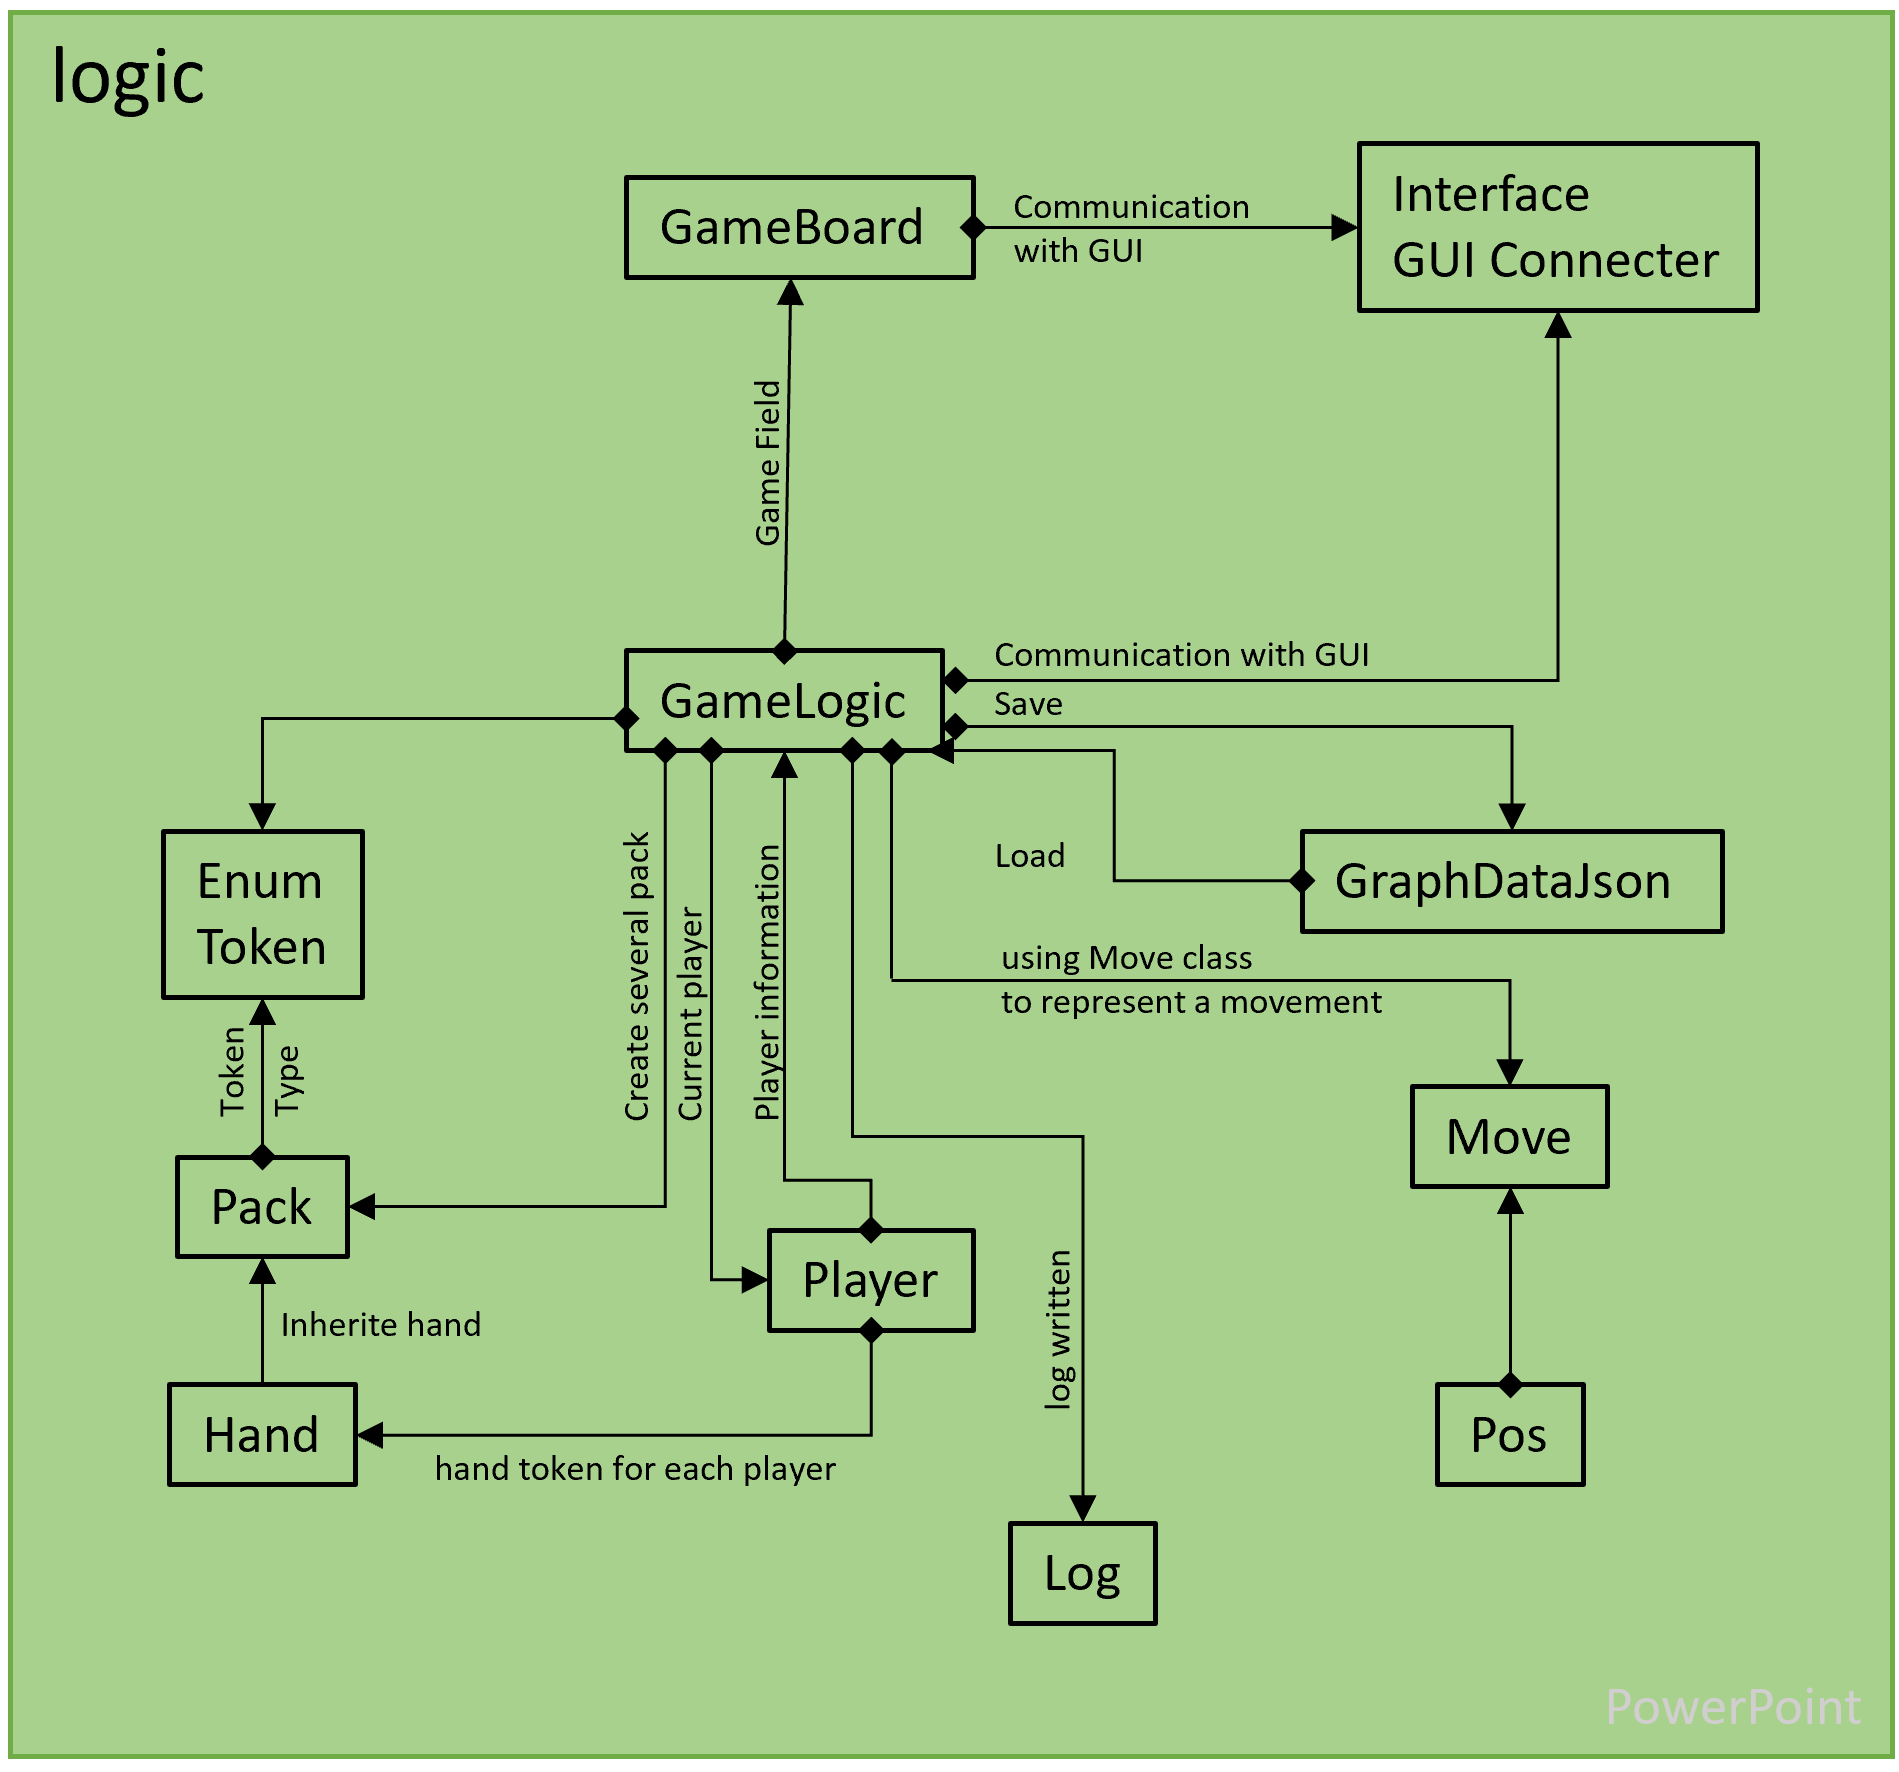
\includegraphics[width=0.8\textwidth]{image/diagram_3}
	\caption{The Logic package}
	\label{fig:logicPackage}
\end{figure}
\subsubsection{Game Logic}


The class Logic is mainly controlled the whole program of the game, the most important core class among it. All other classes will be implemented here and be integrated into the logic of the whole game such as the logic algorithm of the AI, the logic program to determine the winner, and the initialization of the whole game. 

From Figure \ref{fig:gameLogic} below, it is apparent to recognize that the class Logic also needs to communicate bidirectionally with other classes to update some features of the game.

In detail, the class logic frequently interacts with the class player to track the feature of the current player. And lead this feature to the GUI package to display on the main interface in order to become a condition, which is for the participant to realize who needs to play now.   

Additionally, the class Logic also produces an interaction with the class Pack to have a global constant of a full pack, which functions to count the number amount of tokens. Not only does a full pack of all tokens exist but also a pack keeping every action token is required in the program. 
While a token is being used, the token pack needs to be diminished as a used token each time.

Furthermore, as mentioned in the top description, the class Move and the class Position are also being used in some methods of analyzing AI movement.  As a tool, they are generated as an object corresponding to on their class type.


\begin{figure}[h]
	\centering
	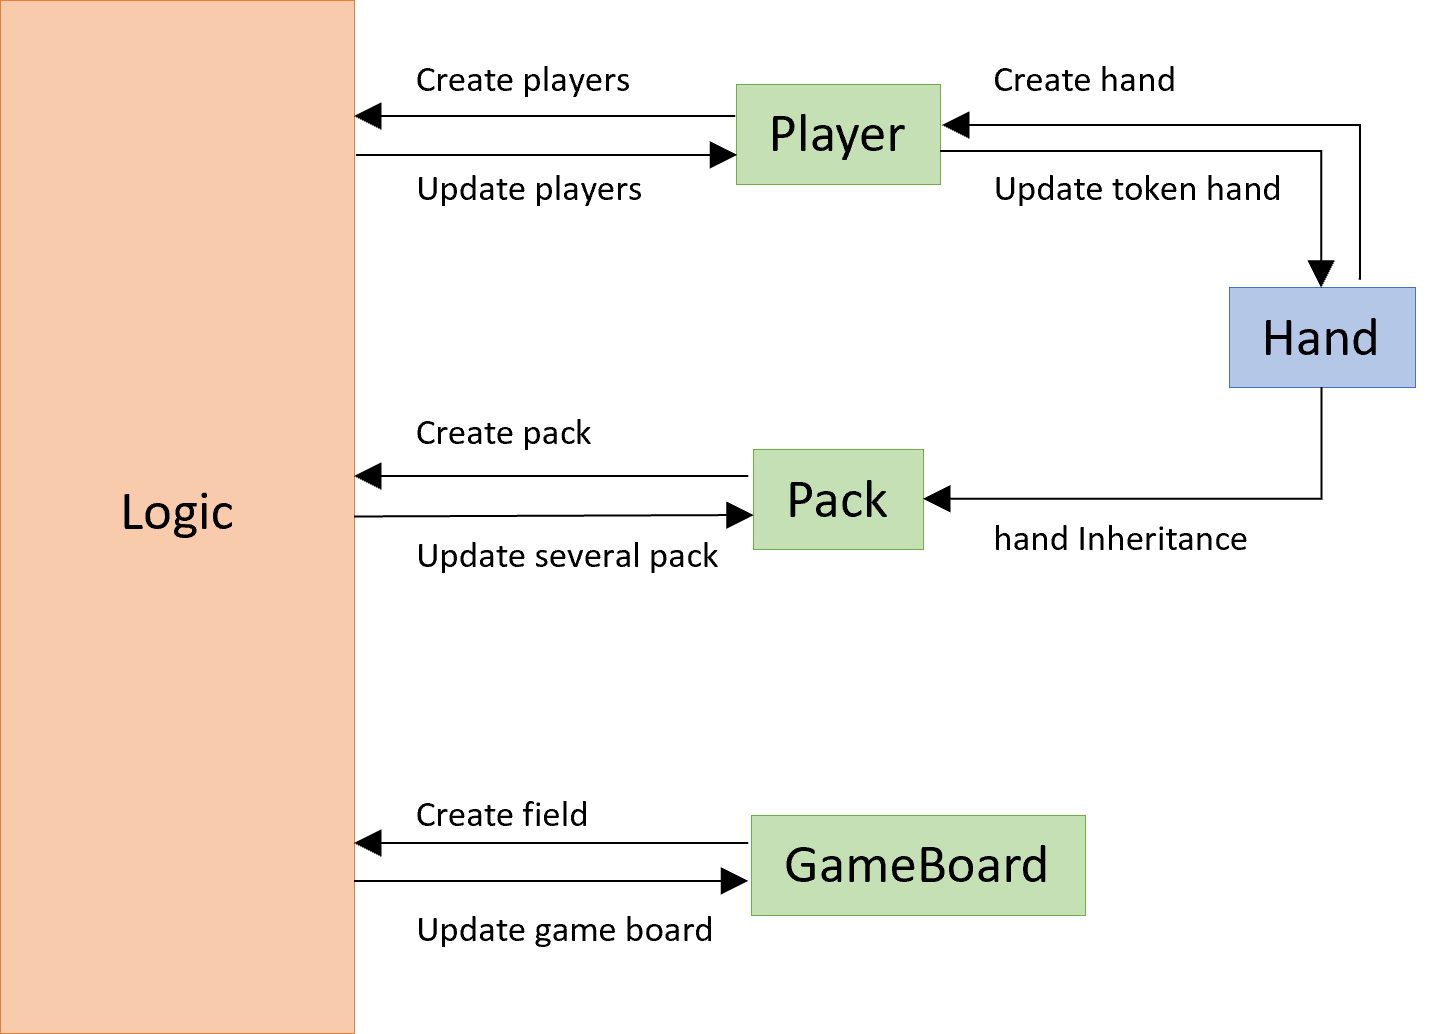
\includegraphics[width=0.8\textwidth]{image/diagram_4}
	\caption{The relationship between GameLogic class and other classes.}
	\label{fig:gameLogic}
\end{figure}


Here has two essential and noticeable developing logics that needs to be mentioned below:

\paragraph{Human} \mbox{}\\
Regards to the logic of the human player playing the game, a few coordinates of the game board and the player's hands are considered the fundamental gist. While a human player uses click or drag action to play the game, the coordinate of those actions needs to be recorded and passed to other functions to accomplish other aims.

\paragraph{AI logic}\mbox{}\\
In the AI logic, it is important to claim that there are some rules that existed in the game. As the turn is in AI, the idea for AI to pick up the best token to get the best score or even attempt to win the game has its own logical design.
In the developmental of our logical design, the two main types of token: Symbol token and Action token are introduced and follow the rules below:   


\begin{enumerate}
	\item\textbf{Winning a game by laying a line of six}\\
    The player should be able to use the token to complete six tokens in a line and win the game. 
This condition is the priority of winning the whole game. However, one thing that needs to realize is that the action token must always be utilized first and then the symbol token is the second option. 
	\item\textbf{Prevent another team to complete six}\\
Since another team has accumulated five tokens in a line on the chess board, the player should be aware of and use tokens to interrupt the possibility of winning the game for another team. Likewise, the action token must be used in advance. 
	\item\textbf{Achieve the best score}\\
	However, achieving the best score has a different arrangement that the symbol token must be considered first when the player has a symbol token on hand. The action token will only be considered when there is no line of six to be completed and there are no symbols token on the player's hand, 
	
\end{enumerate}



\subsubsection{Game board}

A class Game board is represented as a field generated by every token which has been arranged on the chess board. All the methods existing in this class are related to the changes in behaviour or some identified use. It is apparent to observe that the game board class is directly output to the logic class as the player drag and drops a token on the board or modifies some changes. 

\subsubsection{Player}

The class Player aims to create an object player in a game. The object of the player involves several attributes, for instance, the name of the participant, the active state, the AI state, and the hand token for the participant. 
In the constructor of the class logic, the player class can be implemented with the purpose of creating several players for game playing. And also the logic class can keep tracking the current player with the player object.    

\subsubsection{Pack and Hand }

According to the understanding of the game playing, a pack of storing tokens and a hand token of each player is an indispensable element in a game. Hence, with the help of many methods, the class logic can utilize the Class pack to insert, remove or increase tokens in a pack or player's hands. Moreover, because of the inheritance relationship of the class pack and class hand as shown in Figure \ref{fig:packAndHand} below, those methods in the pack class are also applicable to be utilized for hand class. 

\begin{figure}[h]
	\centering
	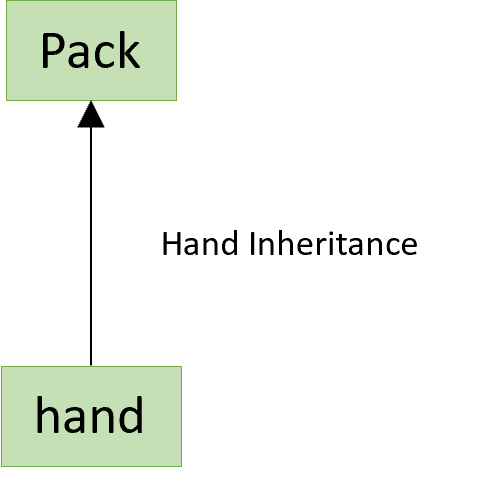
\includegraphics[width=0.3\textwidth]{image/diagram_5}
	\caption{Pack and Hand}
	\label{fig:packAndHand}
\end{figure}

\newpage
\subsubsection{Enum Token }

Regarding the Enum class Token, every token is numbered in an enum category. An advantage of sorting those tokens in the sequence is that other classes are able to invoke the specified token by an ordinal. The sequence of tokens is shown below Figure \ref{fig:enumToken}.

	\begin{figure}[h]
	  \centering
	  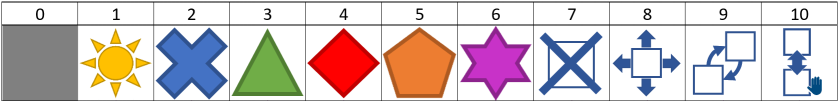
\includegraphics[width=0.8\textwidth]{image/sequenceOfEnumTokens}
      \caption{The sequence of Enum tokens}
	  \label{fig:enumToken}
    \end{figure}

\subsubsection{Move and Position}

The function of the class Move and the class Position is principally the same. Mostly they have a constructor which includes an object to record the necessary attribute and this object can be passed to any class which is required. Indeed, the class Move even contains a position object to perform the movement position as shown in Figure \ref{fig:moveAndPosition} below. Among the position object, it has two attributes x and y, which are the coordinate of the chess board.
  
\begin{figure}[h]
	\centering
	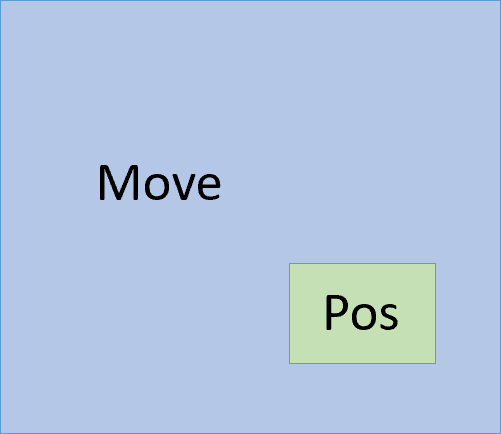
\includegraphics[width=0.3\textwidth]{image/diagram_6}
	\caption{The Move and Position class.}
	\label{fig:moveAndPosition}
\end{figure}


\subsubsection{GraphDataJson}

In this project, the conception of Save and Load is based on the JSON file. To parse a JSON file, GSON is chosen for implementation. And this class contains all information, which is necessary for generating an unfinished game that would be established as a variable in class logic. No matter which operation of Save and Load to use, both of them must through this variable to transform data. The process of transforming data is as below in Figure \ref{fig:GraphDataJson}.      

\begin{figure}[h]
	\centering
	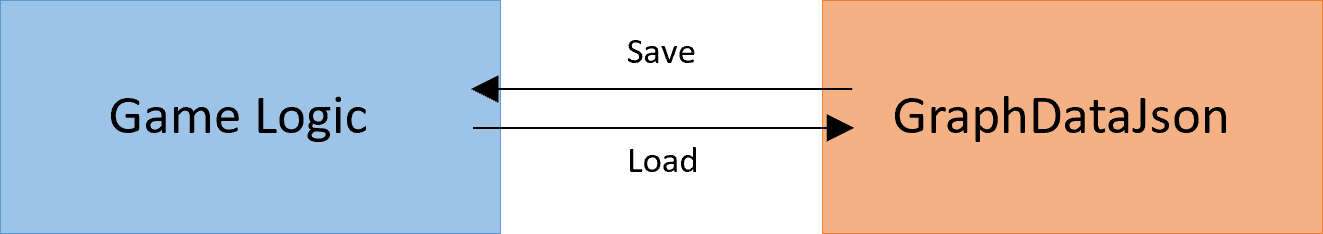
\includegraphics[width=0.6\textwidth]{image/diagram_7}
	\caption{The GraphDataJson class and GameLogic class.}
	\label{fig:GraphDataJson}
\end{figure}